\begin{tabular}{llllllllll}
    \toprule
    \textbf{Model} & \textbf{C} & \multicolumn{2}{c}{\textbf{Server}} & \multicolumn{2}{c}{\textbf{Category}} & \multicolumn{2}{c}{\textbf{Gender}} & \multicolumn{2}{c}{\textbf{Day of week}} \\
    \midrule
    LR-50 & 10 & 36.92 & 52.78 & 33.30 & 72.32 & 43.62 & 69.15 & 18.13 & 19.62 \\
    LR-200 & 100 & 37.27 & 53.38 & 32.77 & 72.69 & 44.06 & 70.52 & 18.34 & 19.83
\end{tabular}

\begin{tabular}{llllllllllll}
    \toprule
    \textbf{Model} & \multicolumn{2}{c}{\textbf{Server}} & \multicolumn{2}{c}{\textbf{Category}} & \multicolumn{2}{c}{\textbf{Gender}} & \multicolumn{2}{c}{\textbf{Day of week}} \\
    \midrule
    R-Base & 69.74 & 78.19 & 54.35 & 79.67 & 51.18 & 74.67 & 29.43 & 29.49 \\
    F-Base & 69.39 & 77.68 & 53.97 & 79.55 & - & - & 29.24 & 29.34 \\
\end{tabular}

\begin{tabular}{l|ll|ll|ll|ll|ll}
    \toprule
    \textbf{Model} & \multicolumn{2}{c}{\textbf{Server}} & \multicolumn{2}{c}{\textbf{Category}} & \multicolumn{2}{c}{\textbf{Gender}} & \multicolumn{2}{c}{\textbf{Day of week}} \\
    \midrule
    R-Base & 69.74 & 78.19 & 54.35 & 79.67 & 51.18 & 74.67 & 29.43 & 29.49 \\
    \midrule
    R-LM & 70.06 & 78.40 & 55.18 & 80.14 & 51.13 & 75.09 & 29.98 & 29.30 \\
    R-Grad-12 & 67.81 & 76.36 & 51.93 & 78.69 & 49.98 & 73.82 & 29.11 & 29.21 \\
    R-Grad-24 & 69.07 & 77.69 & 53.22 & 78.97 & 49.75 & 74.06 & 29.36 & 29.47 \\
    R-Truc & 68.71 & 77.31 & 53.90 & 79.37 & - & - & 29.52 & 29.57 \\
\end{tabular}

% \begin{tabular}{l|ll|ll|ll|ll|ll}
%     \toprule
%     \textbf{Model} & \multicolumn{2}{c}{\textbf{Server}} & \multicolumn{2}{c}{\textbf{Category}} & \multicolumn{2}{c}{\textbf{Gender}} & \multicolumn{2}{c}{\textbf{Day of week}} \\
%     \midrule
%     R-Base & 69.74 & 78.19 & 54.35 & 79.67 & 51.18 & 74.67 & 29.43 & 29.49 \\
%     \midrule
%     R-50 & 
%     F-50 &
%     \midrule
%     GPT-3-50 &
%     \bottomrule
% \end{tabular}

%% Add figure
\begin{figure}[ht]
    \centering
    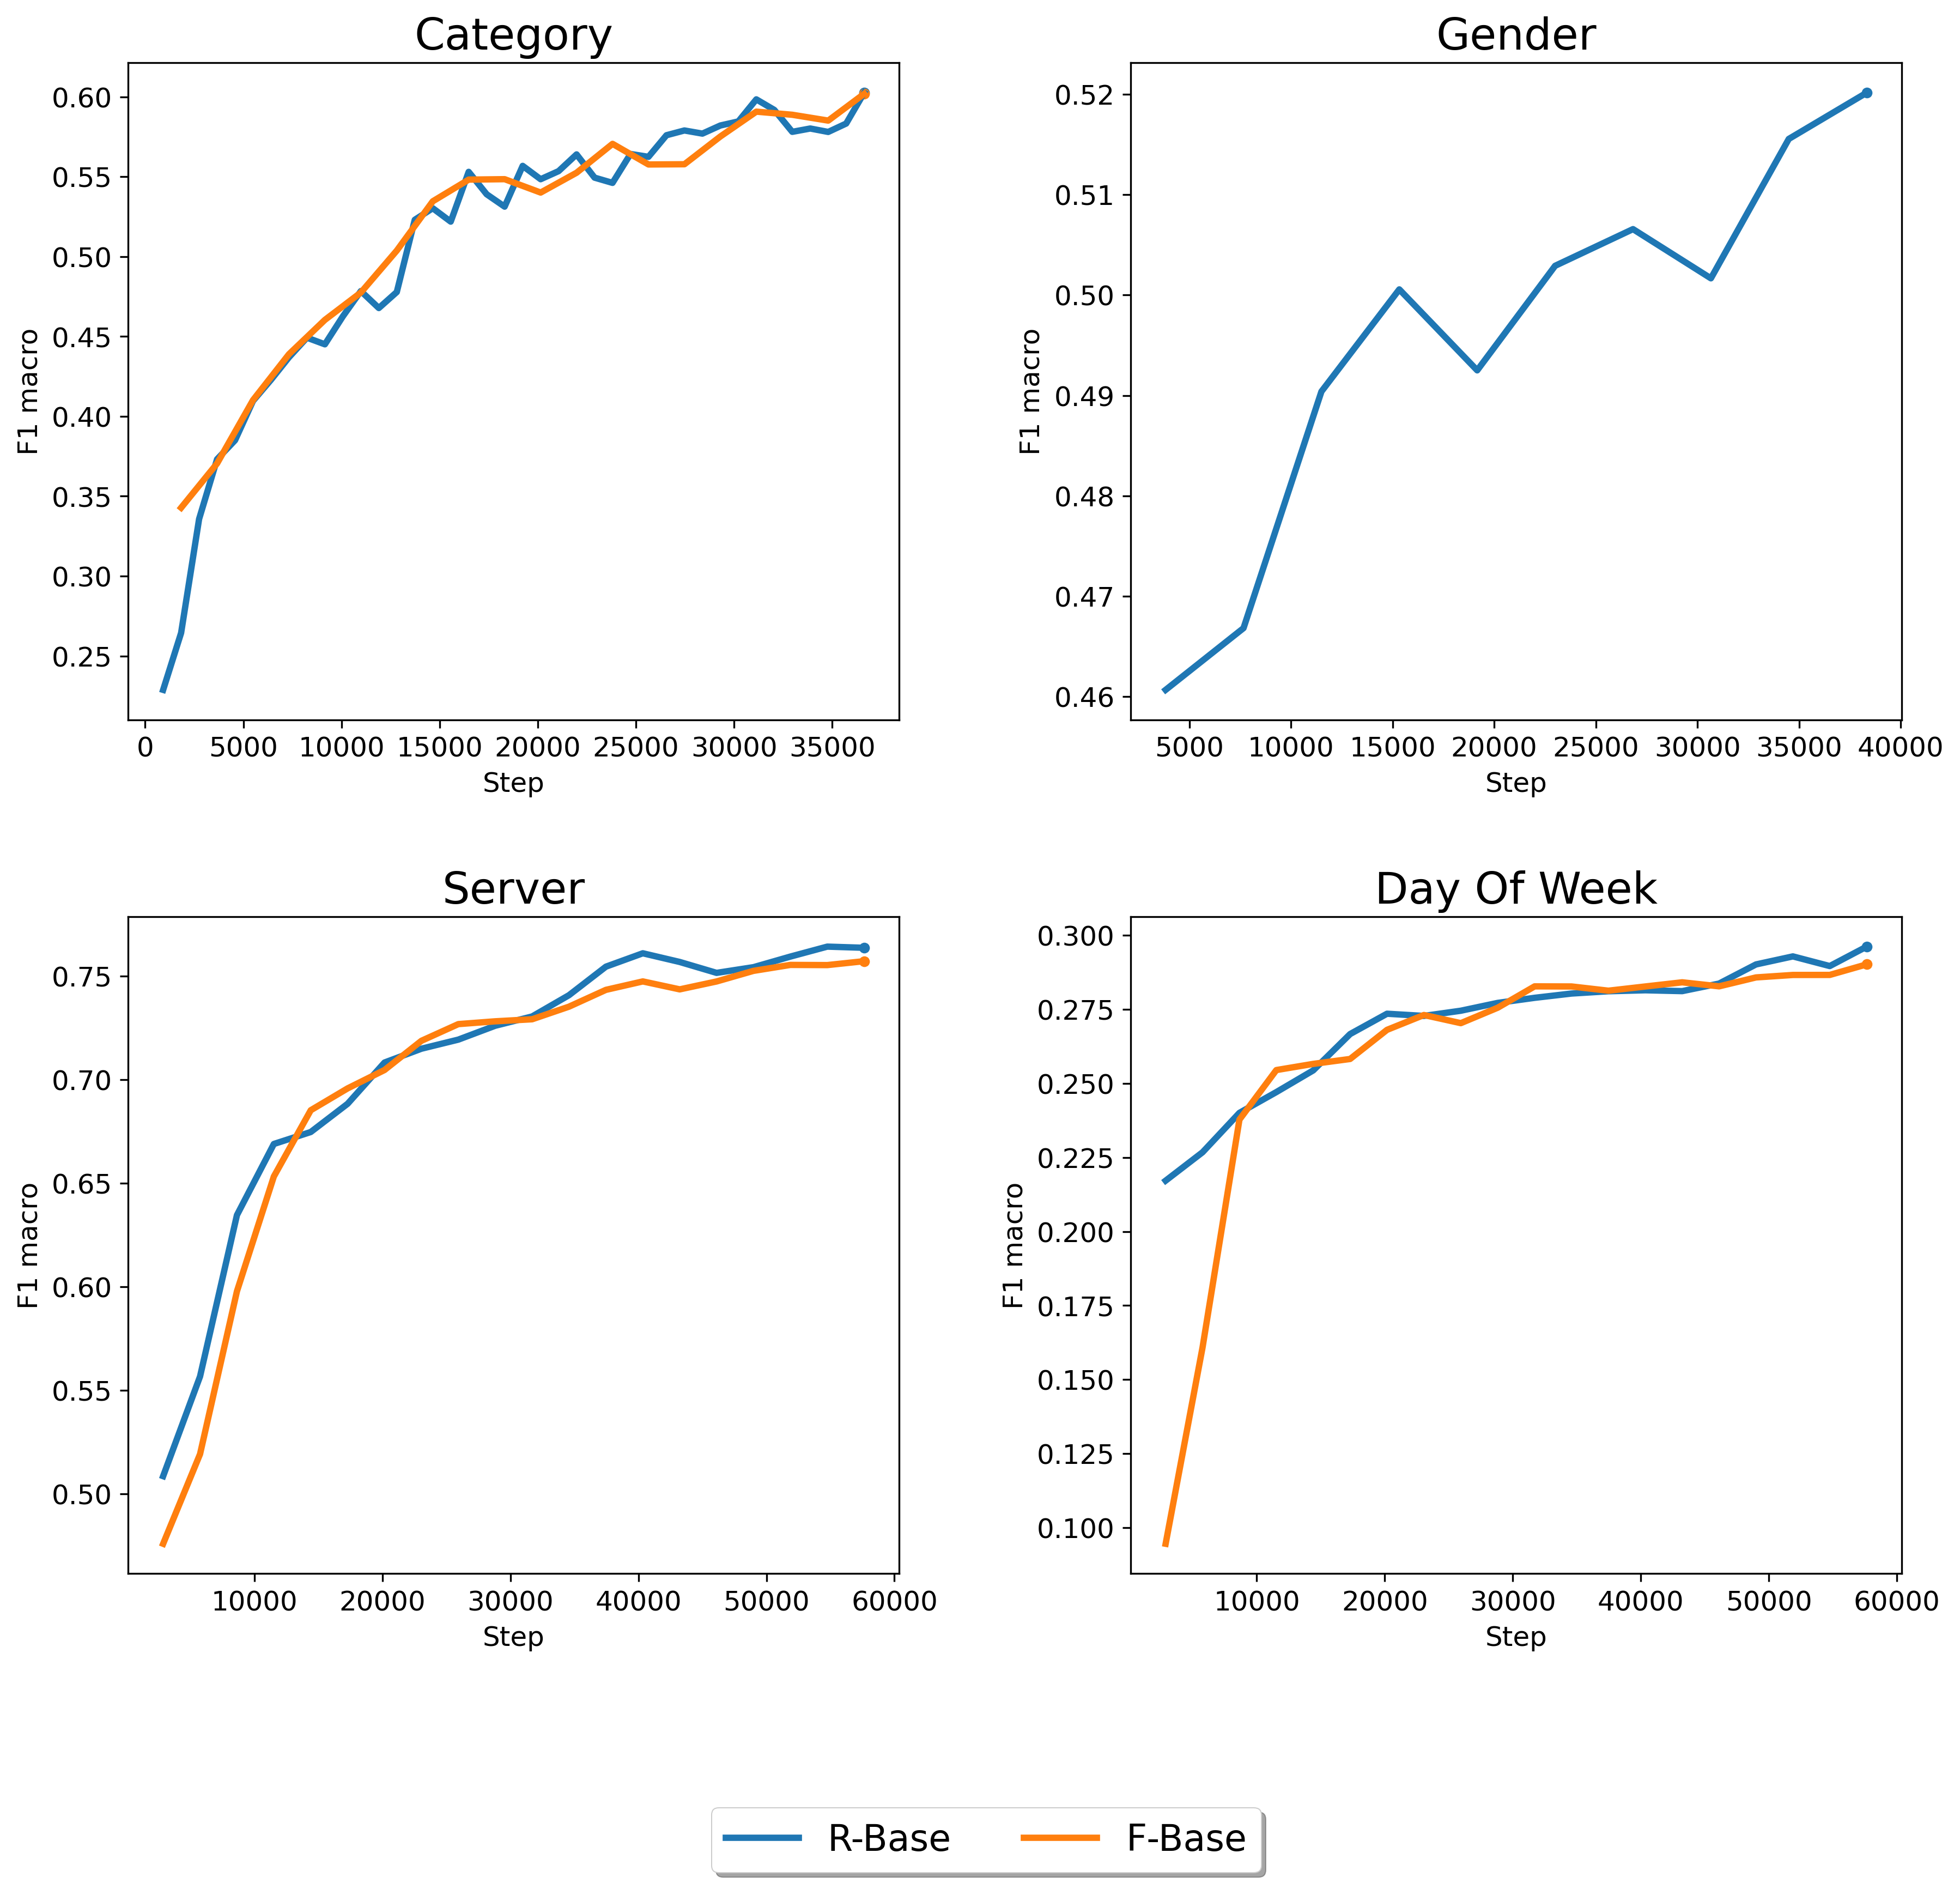
\includegraphics[width=0.8\textwidth]{graph_create/outputs/base.png}
    \caption{Caption}
    \label{fig:base-train}
\end{figure}

\begin{figure}[ht]
    \centering
    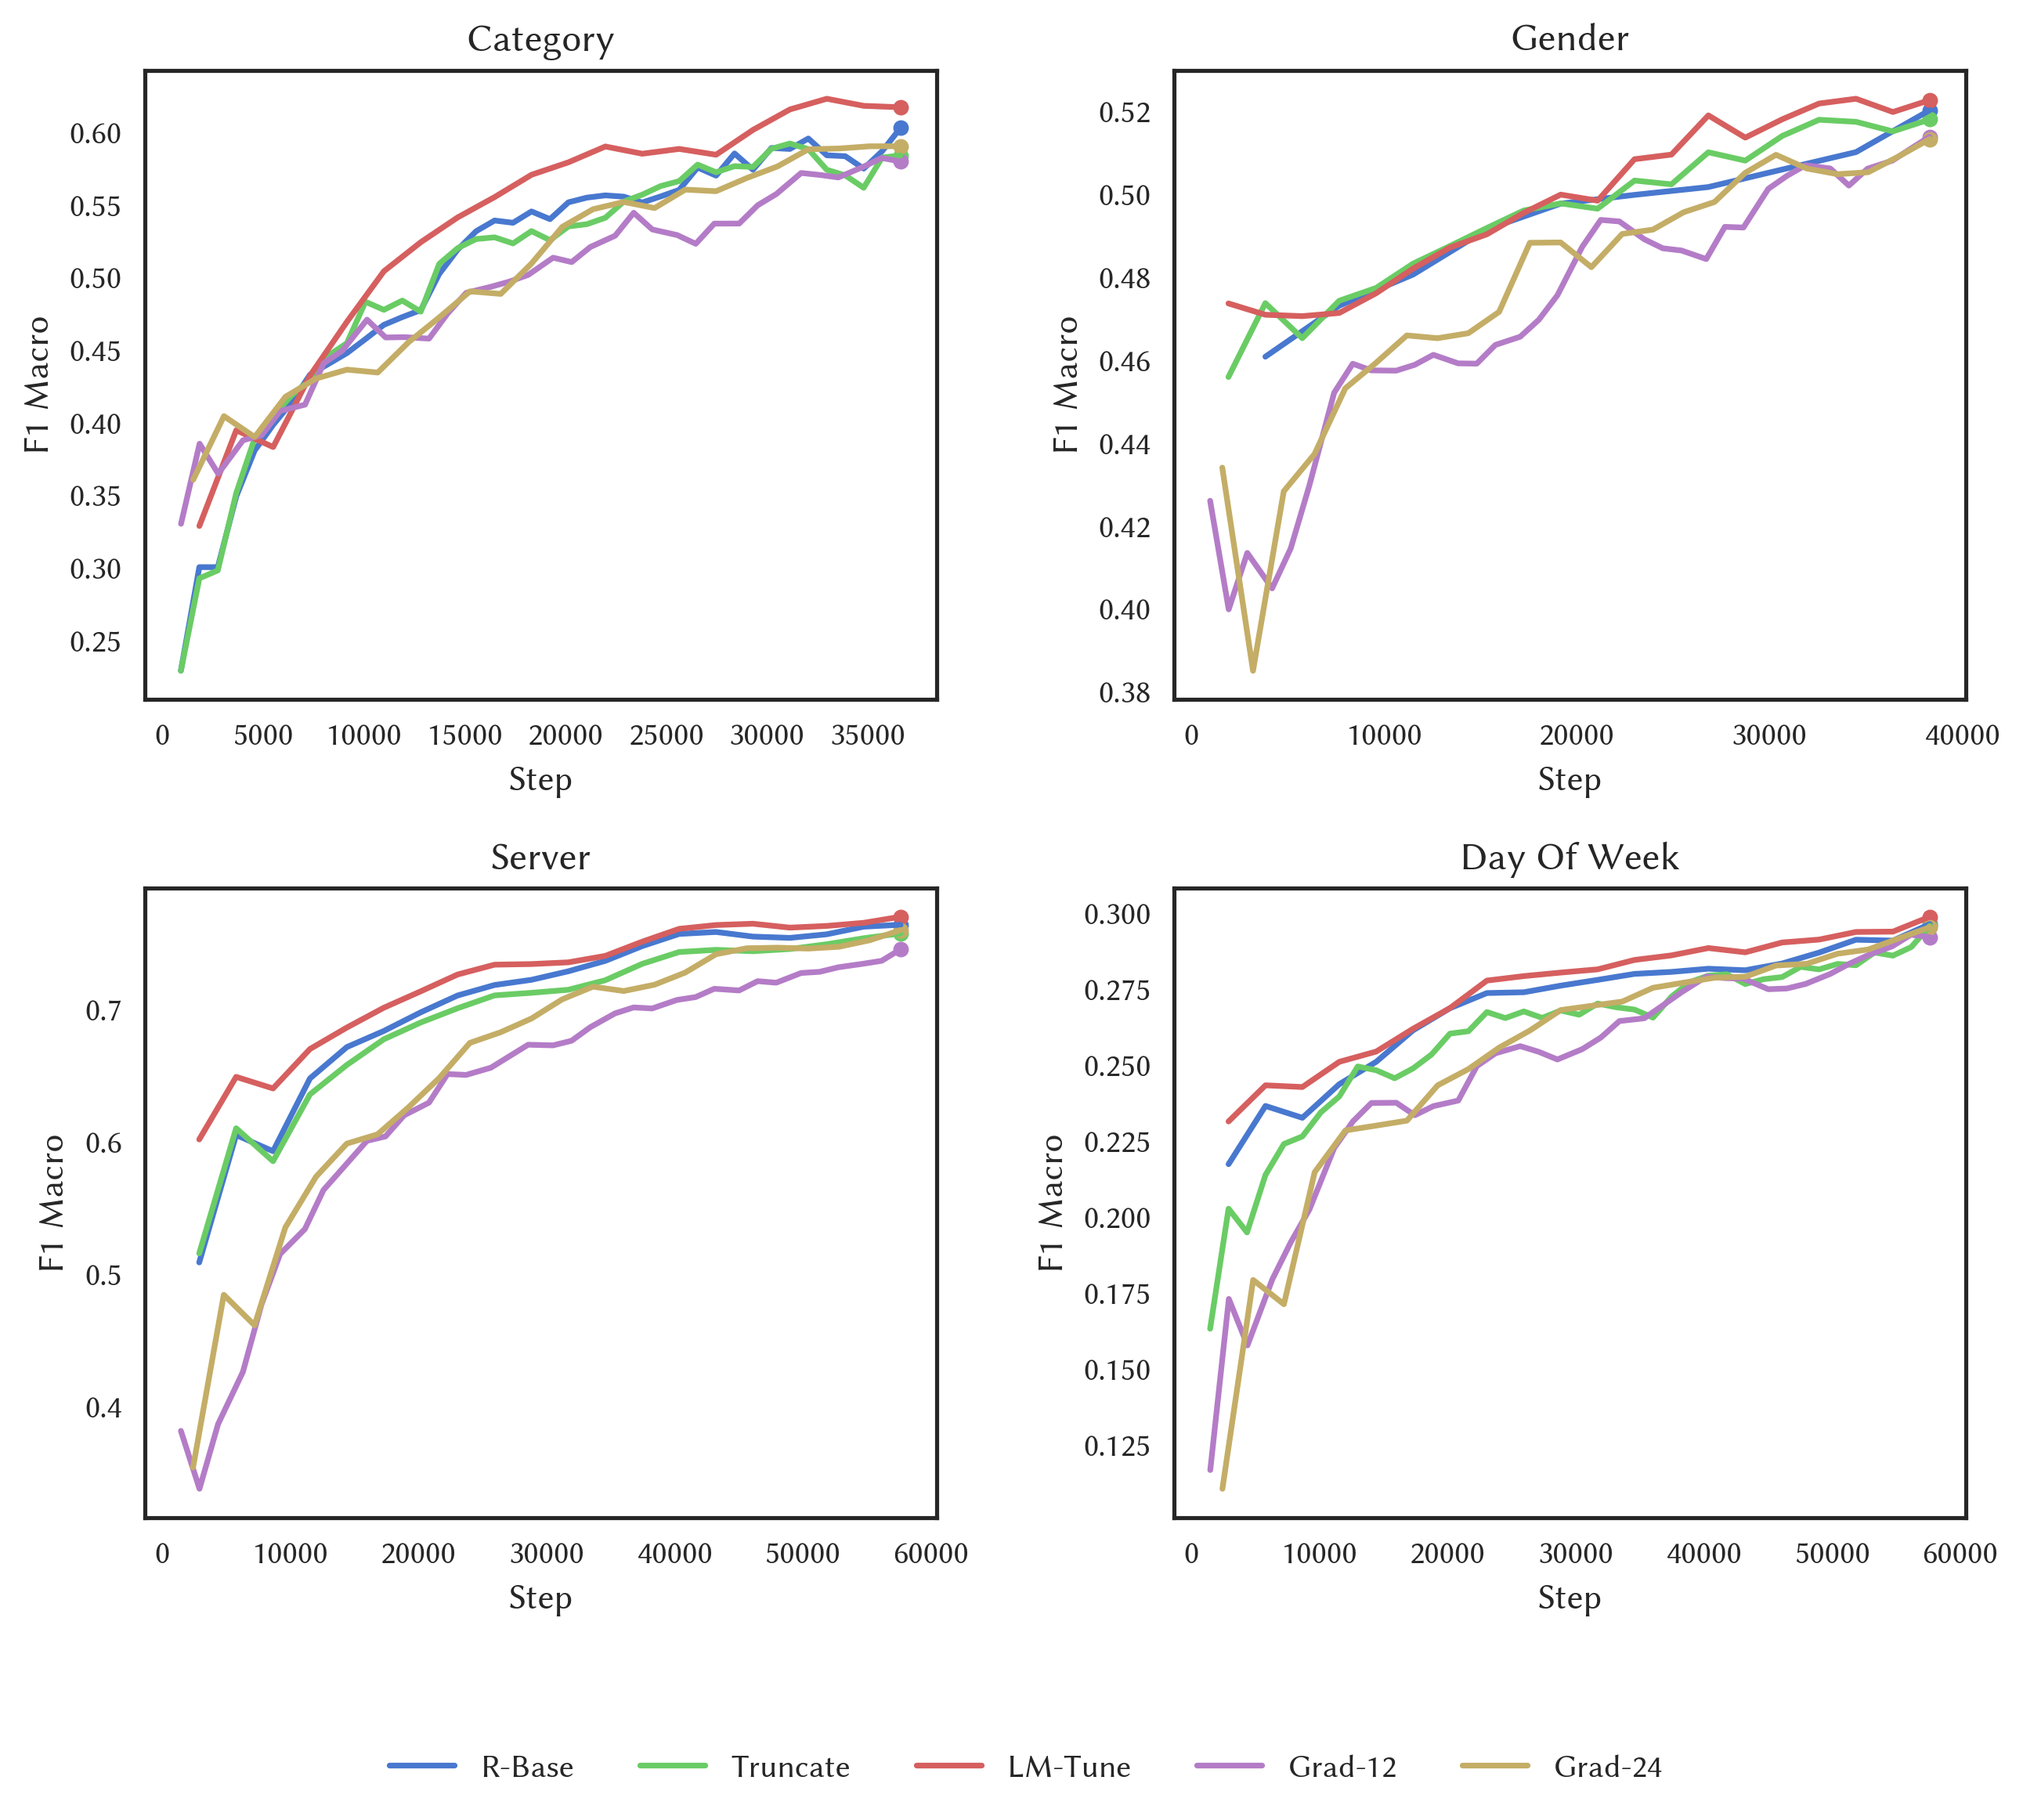
\includegraphics[width=0.8\textwidth]{graph_create/outputs/tune.png}
    \caption{Caption}
    \label{fig:tune-train}
\end{figure}


\section{Baseline}
\label{sec:baseline}
We haven't observed significant improvement by adding 150k additional features.
While both metrics have improved across all but categories, the improvement is
less than less than $1\%$. 
We also observed the most significant features for each task and class and
haven't found much of a difference between the two models.
We thus only show the features for LR-200 in \autoref{tab:tfidf-features}.
The significant feature are mostly unsuprising. For day of week the model
found the name days to be significant. The categories features are
connected to category names, we can also see the category overlap
as disscued in \autoref{sec:category}. For server task we observe
that the actual server names can be found in documents, however
this issues is not widespread as the metrics would otherwise be much
higher suggesting task to be trivial. As for genders we couldn't
find any interpretation for keywords.


\section{Backbone models}
The transformer models clearly beat the simple baseline across all tasks
with imprvoments going as far as $33\%$ it's thus clear that the context
significantly matters.

As for RobeCzech and Fernet comparisoing have observed RobeCzech bearing the Fernet model
across the tasks. During training, we had hard time with training the Fernet model
we had to lower lr a lot so that the model wouldn't start diverging early at the training.
As for the Gender task the model diverge even for lr of $9*10^{-6}$,
we thus haven't tried further.
These resuls rather surprised us. We hoped that due to the pretraining data domain
being the same as ours, the Fernet model would have better pretrained weights
and more alligned Embeddings which would allow large parts of text to be embeded.
This however didn't happen as the observed results show.
In fact average characeters per token for RobeCzech: $4.68$, Fernet: $4.46$, GPT-3: $1.77$
The GPT-3 values are due to model being multi-lingual.

As for gpt3 comparison we were fairly suprised that even while being purely generative
and trained in multi-task setting managed to correctly output the respective classes in all cases.
While performance clearly haven't beaten the models, it is still a good result.
For reference the 

We have been suprised by model performances considering the fact that they have been trained
on 1/20 size of original dataset. 


\section{Finetuning}
We haven't found much success with finetuning approaches.
The only consistent helpful modification was LM-tuning.

As for Gradual Unfreezing we found similar results to \todo{cite},
it's possible that GU would allow for highger learning rates, but we haven't
investiaged further

\section{Final model}
As the only helpful finetuing approach was LM we only used it for final model creation.
Due to realtive success of short model training we further used following modifications
\begin{enumerate}
    \item Lower warmup steps: 0.1 -> 0.01
    \item Most recent sampling: As the short training showed, it's likely
    that most recent 
\end{enumerate}
\todo{Evaluate final models more in depth}





\begin{table}
\centering
\caption{Top 4 features for Category}
\label{tab:top4_category}
\begin{tabular}{lcccc}
\toprule
{} &               1 &                2 &              3 &               4 \\
\midrule
Domácí         &         mf dnes &     radiožurnálu &       idnes.cz &           klaus \\
Sport          &         fotbalu &              nhl &        turnaji &           kluby \\
Zahraniční     &             osn &          . úřady &      : reuters &   vyšetřovatelé \\
Kultura        &           album &               čt &       koncertu &          snímek \\
Ekonomika      &           banka &         analytik &            řsd &       ekonomiky \\
Krimi          &  mluvčí policie &       řekl právu &  miliónů korun &     řekla právu \\
Technologie    &           herní &               pc &        windows &           . hra \\
Koktejl        &            miss &         novinkám &          daily &        zpěvačka \\
Životní styl   &        sexuální &       university &            sex &            sexu \\
Auto           &     automobilky &       automobilů &          motor &              kw \\
Věda           &           vědci &       vzdělávání &        fakulty &         školách \\
Komentáře      &             . ) &           babiše &   andrej babiš &          zemana \\
Cestování      &         turistů &          turisté &              — &   profimedia.cz \\
Finance        &            bank &        pojištění &          banka &      pojišťovny \\
Podnikání      &     úřadu práce &              okd &       pivovaru &           horal \\
Bydlení        &       interiéru &        architekt &            . : &            vily \\
Koronavirus    &      koronaviru &      koronavirem &    koronavirus &      nakažených \\
Byznys         &           akcie &              čez &  zaměstnavatel &       meziročně \\
Rozhovory      &           videu &            výzvě &    ? podívejte &       podívejte \\
Podcasty       &               〜 &                ■ &    poslechněte &  poslechněte si \\
Revue          &         herečka &         zpěvačka &        modelka &           herec \\
Literatura     &           román &   nakladatelství &          kniha &          románu \\
Vánoce         &          vánoce &            dárky &      vánočních &         cukroví \\
Výtvarné umění &         galerie &  národní galerie &          obraz &             děl \\
Kolo           &               〜 &         cyklisty &       cyklisté &        cyklistů \\
\bottomrule
\end{tabular}
\end{table}

\begin{table}
\centering
\caption{Top 4 features for Day of week}
\label{tab:top4_day_of_week}
\begin{tabular}{lcccc}
\toprule
{} &            1 &                2 &               3 &                 4 \\
\midrule
MONDAY    &     pondělní &     pondělí ráno &  minulého týdne &    pondělí mluvčí \\
TUESDAY   &       úterní &       úterý ráno &        úterního &          pondělní \\
WEDNESDAY &    středeční &           úterní &     středu ráno &       řekl středu \\
THURSDAY  &    čtvrteční &     čtvrtek ráno &       středeční &         . čtvrtek \\
FRIDAY    &   pátek ráno &     příští týden &         páteční &         čtvrteční \\
SATURDAY  &  sobotu ráno &          páteční &    příští týden &  sobotu dopoledne \\
SUNDAY    &      nedělní &  václava moravce &     neděli ráno &          sobotním \\
\bottomrule
\end{tabular}
\end{table}

\begin{table}
\centering
\caption{Top 4 features for Server}
\label{tab:top4_server}
\begin{tabular}{lcccc}
\toprule
{} &             1 &              2 &             3 &                 4 \\
\midrule
seznamzpravy &         videu &  seznam zprávy &     podívejte &            ” říká \\
idnes        &      idnes.cz &        mf dnes &      více zde &        více čtěte \\
aktualne     &   aktuálně.cz &        praha – &       video : &            brno - \\
novinky      &    řekl právu &  miliónů korun &      novinkám &           , právo \\
denik        &    čtěte také &       deníku . &   řekl deníku &                 ­ \\
irozhlas     &  radiožurnálu &    radiožurnál &  \&\#124; zdroj &  českého rozhlasu \\
\bottomrule
\end{tabular}
\end{table}

\begin{table}
\centering
\caption{Top 4 features for Gender}
\label{tab:top4_authors_cum_gender}
\begin{tabular}{lcccc}
\toprule
{} &                 1 &        2 &           3 &               4 \\
\midrule
MAN   &  důchodový systém &   důkazy &  důchodců a &  \&quot; kroutil \\
WOMAN &               epa &  došlých &  elektricky &           etapu \\
MIXED &            band . &  dějství &     děkanka &            bili \\
\bottomrule
\end{tabular}
\end{table}